\scanpage{27}
% Full-page vertical rules are anchored to the first and last entries below.
\noindent\tikz[remember picture,overlay]{\coordinate(sc27Ctop);}%
\unsure{302}\tikz[remember picture,overlay]{\coordinate(sc27Clefttop);} l.15 ``its

303 l.1 ``\deleted{\unsure{with|who}} which will be'' l2 ``we've got'' l.-3 ``image of $A$ by $A$'' - not clear what you mean.

304 l-15 ``commutes with'' also l-13. \deleted{\unsure{l-2} ``play'' \unsure{no|not} ``s}''

305 l.5 ``interpret' l14 ``commutes with''

306 l.19 ``its'' \deleted{l} also l-5. l-4 ``test \uline{category}''

309 l.-8 ``on \uline{the} previous''

312 l-.8 ``isn't'' \deleted{l-6 \unsure{lets|let's}}

313 l9 'shouldn't'' l.18 ``don't'' l-12 ``commutes with''

\deleted{filtering \raisebox{.7ex}[0pt][0pt]{\unsure{out|at|on|or}}} \unsure{l-2|l-7} filtering''

314 l.5 ``isn't'' l.6 ``as is''

315 Sent\tikz[baseline=(sc27Csentence.base)]{\node[inner sep=0pt] (sc27Csentence) {\deleted{\unsure{ann|en}}};\node[anchor=base west,inner sep=0pt] at ([yshift=.1ex]sc27Csentence.base west) {en};}ce starting l.7 - difficult to understand. Possibly: 'I add this comment, of course, \deleted{to} in order to ``\uline{push home}'' the point that \uline{no more} with resp... than in any other essential respect. concerning the ability \uline{to express} basic situations.....theory, \uline{does} the cat. ... \uline{stand} singled out. \deleted{(This is \raisebox{1.1ex}[0pt][0pt]{\makebox[0pt][l]{\inserted{certainly}}}true \raisebox{1.1ex}[0pt][0pt]{\makebox[0pt][l]{\inserted{as far as our}}}\unsure{presumably} at the present knowledge goes). \unsure{No|Now} \textendash{}\,\textendash{}.} (This certainly seems to be so as far as our present knowledge goes)''...

l.17 ``its'' l.-3 'and which \tikz[baseline=(sc27Cwouldbase.base)]{\node[inner sep=0pt,minimum width=.25em] (sc27Cwouldbase) {\strut};\node[anchor=south west,inner sep=0pt] at ([yshift=.9ex]sc27Cwouldbase.base west) {\inserted{would}};\draw ([xshift=.08em,yshift=-.65ex]sc27Cwouldbase.base west) -- ([xshift=.16em,yshift=-.25ex]sc27Cwouldbase.base west) -- ([xshift=.26em,yshift=-.5ex]sc27Cwouldbase.base west);} allow one to compute''

316. l.1 ``shouldn't'' l12 ``$i(a)$ \deleted{it} is a ''\deleted{\unsure{to|is}}

317. l.11 'its'' l-16 \unsure{``|'}isn't''

320 l 8. ``indispensable'' l-15 'developing'' l-8 ``its''

321 l.9 'isn't''

323 l13 ``don't''

326 l-12 \deleted{\&} \& l.-8 \tikz[remember picture,overlay]{\coordinate(scxxviim);\node[anchor=south west,inner sep=0pt] at ([xshift=.2em,yshift=1.4ex]scxxviim) {\inserted{\& l-3}\tikz[baseline=0pt,x=1ex,y=1ex]{\fill (.07,.7) circle (.035);}};} ``commutes \uline{with}'' and

p.327. l7 ``$\alpha:\mathord{\tikz[baseline=0pt,x=1ex,y=1ex]{\draw[line width=.085ex,line cap=round,line join=round] (.19,0)--(.86,1.37)--(1.08,0)--(.71,.025) (.61,.032)--(.19,0) (-.05,.08)--(.51,1.12);}}\tikz[remember picture,overlay]{\coordinate(scxxviin); \draw ([xshift=.2em]scxxviim) -- ([xshift=.4em,yshift=1.3ex]scxxviin); \draw ([xshift=.57em,yshift=1.7ex]scxxviin) -- ([xshift=.67em,yshift=1.4ex]scxxviin) -- ([xshift=.77em,yshift=1.6ex]scxxviin);}\longrightarrow \mathord{\tikz[baseline=0pt,x=1ex,y=1ex]{\draw[line width=.085ex,line cap=round,line join=round] (.20,0)--(.83,1.12)--(1.22,.05)--(.82,.04) (.72,.02)--(0,0)--(.64,.99);}}/F$'' should it be '

l-17 ``allows \uline{one} to'' l-16 ``doesn't'' l-14 ``isn't\deleted{''} there!''

l-5 ``don't''

p328 l-12 \deleted{wouldn't} should ``wouldn't'' = ``shouldn't''

l-10 doesn't

p329 l.6 $\mathord{\tikz[baseline=0pt,x=1ex,y=1ex]{\draw[line width=.09ex,line cap=round,line join=round] (.16,-.05)--(.77,1.5)--(1.21,.04)--(.16,.0) (.49,1.36)--(-.04,0)--(.21,0);}}$ (doubled side is missing) ``its''

l12 ``don't'' l-13 ``makes sense'' l.-13 \unsure{``|'}semisimplicial\unsure{,|.} \tikz[remember picture,baseline=0pt,x=1ex,y=1ex]{\coordinate(sc27C329addition);\draw (0,-.6)--(.45,1.7); \draw (.14,.1)--(.43,-.1);\node[anchor=south west,inner sep=0pt] at (-.75,2.1) {\inserted{l-5. ``enveloping\unsure{'|''}}};\fill (-.25,4.8) circle (.035);\fill (-.18,5.1) circle (.03);}\normalmarginpar\margin{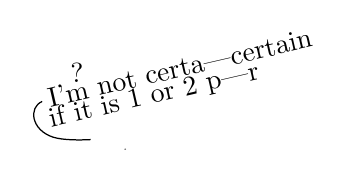
\begin{tikzpicture}[x=1em,y=1ex,baseline=0pt]
\node[anchor=west,inner sep=0pt] at (.8,3.2) {?};
\node[anchor=west,inner sep=0pt,rotate=13] at (0,1.1) {I'm not \unsure{certa|certain}};
\node[anchor=west,inner sep=0pt,rotate=13] at (.05,-.8) {if it is 1 or 2 \unsure{p|r}};
\draw[line width=.45pt] (-.2,.8) .. controls (-.7,.3) and (-.6,-1.6) .. (.2,-2.2) .. controls (.55,-2.45) and (1.15,-2.45) .. (1.55,-2.4);
\fill (2.8,-3.2) circle (.035);
\end{tikzpicture}}
% slanted; right edge of the note is clipped

p.333 l.-12 ``makes sense''

\noindent\tikz[remember picture,overlay]{\coordinate(sc27Cbottom);}p.334\tikz[remember picture,overlay]{\coordinate(sc27Cleftbottom);} l.3 '$b\in A_{n-1}$'' l-6 ``its'' also in l-5.

% Vertical rules, at the observed sides of the list; not a detached drawing panel.
\tikz[remember picture,overlay]{
\draw[line width=.3pt] ([xshift=.45em,yshift=1.3ex]sc27Clefttop) -- ([xshift=.05em,yshift=-2.6ex]sc27Cleftbottom);
\draw[line width=.3pt] ([xshift=.93\linewidth,yshift=1.1ex]sc27Ctop) -- ([xshift=.935\linewidth,yshift=-2.8ex]sc27Cbottom);
}
% archive sheet number: 26
